\documentclass[serif,9pt]{beamer}
\usetheme{tree}
%\usepackage{german}
\usepackage[latin1]{inputenc}
\usepackage[spanish]{babel}

% Images
\usepackage{graphicx}
\usepackage{subfigure} % subfiguras
\usepackage{caption}
\usepackage{float}
\captionsetup[table]{labelformat=empty}
\captionsetup[figure]{labelformat=empty}

\usepackage{amsmath}

\usepackage{listings}
\lstset
{ %Formatting for code in appendix
  language=C++, % choose the language of the code
  basicstyle=\fontfamily{pcr}\selectfont\footnotesize\color{black},
  keywordstyle=\color{darkorange}\bfseries, % style for keywords
  numbers=left, % where to put the line-numbers
  numberstyle=\tiny, % the size of the fonts that are used for the line-numbers     
  backgroundcolor=\color{white},
  showspaces=false, % show spaces adding particular underscores
  showstringspaces=false, % underline spaces within strings
  showtabs=false, % show tabs within strings adding particular underscores
  tabsize=2, % sets default tabsize to 2 spaces
  captionpos=b, % sets the caption-position to bottom
  breaklines=false, % sets automatic line breaking
  breakatwhitespace=false, 
}

\AtBeginSection[]
{
  \begin{frame}<beamer>{Contenido}
    \tableofcontents[currentsection]
  \end{frame}
}

\definecolor{darkorange}{rgb}{0.94,0.4,0.0}

\begin{document}
\setbeamertemplate{navigation symbols}{}

\title{Pr�ctica 3: Algoritmos Greedy}  
\author{David Cabezas Berrido\\ Patricia C�rdoba Hidalgo\\ Emilio Hoyo Medina\\ Inmaculada Mar�n Carballo}
\date{}

\begin{frame}
\titlepage
\end{frame}

\begin{frame}\frametitle{�ndice}\tableofcontents
\end{frame}

\section{Introducci�n}
\begin{frame}\frametitle{Introducci�n}
El problema del viajante de comercio (TSP) consiste en encontrar el
ciclo hamiltoniano de peso m�nimo en un grafo conexo y ponderado. En
esta pr�ctica intentaremos abordar este problema por tres algoritmos
greedy distintos.
\end{frame}

\subsection{Enfoque Greedy}

\begin{frame}\frametitle{Enfoque Greedy}
\begin{enumerate}
\item \textbf{Conjunto de candidatos:} Las distintas ciudades a
  recorrer, que ser�n los nodos del grafo.
\item \textbf{Candidatos ya usados:} Ciudades ya a�adidas al ciclo.
\item \textbf{Criterio soluci�n:} Una permutaci�n del conjunto de
  ciudades es soluci�n.
\item \textbf{Criterio factible:} Cualquier lista de ciudades (no
  repetidas) puede llegar a ser soluci�n.
\item \textbf{Funci�n de selecci�n:} A determinar por el algoritmo.
\item \textbf{Funci�n objetivo:} A un ciclo soluci�n le asocia la suma de los pesos de las aristas de dicho ciclo (debemos minimizarla).
\end{enumerate}
\end{frame}

\section{Algoritmos}

\subsection{Algoritmo del vecino m�s cercano}

\begin{frame}
  \begin{center}
    \Huge Algoritmo del vecino m�s cercano
  \end{center}
\end{frame}

\begin{frame}[fragile]\frametitle{C�digo}
  \begin{lstlisting}
  vector<int> result(n);
  result[0] = 0;

  int dmin;
  int sumDistances=0;
  for(int k = 1; k < n; k++){
    dmin = INT_MAX;

    for(j = 0; j < n; j++)
      if(find(result.begin(),result.end(),j) == result.end()){
        distance = map[max(j,result[k-1])][min(j,result[k-1])];
        if(distance < dmin){
          i = j;
          dmin = distance;
        }
      }
    sumDistances += dmin; 
    result[k] = i; 
  }
  
  sumDistances += map[max(result[0],result[n-1])] 
                     [min(result[0],result[n-1])]; 
\end{lstlisting}
\end{frame}

\begin{frame}\frametitle{Eficiencia Te�rica}
  Despreciando las constantes, el c�lculo de la eficiencia es:
  $$n*\sum_{k=1}^{n}k = n*\frac{(n+1)*n}{2} = \frac{n^3+n^2}{2}$$
  Eficiencia: $O(n^3)$ \\
  % \vspace{2mm}
  % Donde:\\
  % k: tama�o del vector result (find)\\
  % n: tama�o del vector candidates
\end{frame}

\subsection{Algoritmo de insercci�n}

\begin{frame}
  \begin{center}
    \Huge Algoritmo de insercci�n
  \end{center}
\end{frame}

\begin{frame}[fragile]\frametitle{C�digo}
  \begin{lstlisting}
while(candidates.size()>0){
  for(i = 0; i < candidates.size(); i++){
    bestD = INT_MAX;
    for(j = 0; j < result.size(); j++){
      d = map[max(result[j],candidates[i])][min(result[j],candidates[i])]
      + map[max(result[(j+1)%result.size()],candidates[i])]
           [min(result[(j+1)%result.size()],candidates[i])]
      - map[max(result[(j+1)%result.size()],result[j])]
           [min(result[(j+1)%result.size()],result[j])];
      if(d < bestD){
        bestCity = candidates[i];
        bestPosition = (j+1)%result.size();
        bestD = d;
      }
    }
  }
  result.insert(next(result.begin(),bestPosition),bestCity);
  candidates.erase(remove(candidates.begin(),candidates.end(),bestCity)); 
  sumDistances += bestD;
}
  \end{lstlisting}
\end{frame}

\begin{frame}\frametitle{Eficiencia Te�rica}
\begin{align*}
\sum_{k=1}^{n}(k((n-k)+1)+n)&=\sum_{k=1}^{n}kn-\sum_{k=1}^{n}k^2+\sum_{k=1}^{n}k+\sum_{k=1}^{n}n\\&=n(\frac{n(n+1)}{2})-\frac{n(n+1)(2n+1)}{6}+\frac{n(n+1)}{2}+n^2\\&=\frac{3n^3+3n^2}{6}-\frac{2n^3+3n^2+n}{6}+\frac{n(n+1)}{2}+n^2\\&=\frac{n^3-n}{6}+\frac{n(n+1)}{2}+n^2
\end{align*}
  Eficiencia: $O(n^3)$
\end{frame}

\subsection{Nuestro Algoritmo: Double Nearest}
\begin{frame}
  \begin{center}
    \Huge Nuestro Algoritmo: Double Nearest
  \end{center}
\end{frame}

\begin{frame}[fragile]\frametitle{C�digo}
  \begin{lstlisting}
for(int k = 1; k < n/2; k++){
  bestD = INT_MAX;
  for(i = 0; i < candidates.size(); i++){
    d1 = map[max(candidates[i],result[2*k-2])]
            [min(candidates[i],result[2*k-2])];
    d2 = INT_MAX;
    for(j = 0; j < candidates.size(); j++){
      if(candidates[j] != candidates[i]){
        d2 = map[max(candidates[i],candidates[j])]
                [min(candidates[i],candidates[j])];
        if(d1 + d2 < bestD){
          bestD = d1 + d2;
          bestCity1 = candidates[i];
          bestCity2 = candidates[j];
        }}}}
  result[2*k-1] = bestCity1;
  result[2*k] = bestCity2;
  sumDistances += bestD;
  candidates.erase(remove(candidates.begin(),candidates.end(),bestCity1));
  candidates.erase(remove(candidates.begin(),candidates.end(),bestCity2));
}
  if(!(n%2)){
    result[n-1] = candidates[0];
    sumDistances += map[max(result[n-1],result[n-2])]
                       [min(result[n-1],result[n-2])];
  }
  \end{lstlisting}
\end{frame}

\begin{frame}\frametitle{Eficiencia Te�rica}
  \begin{align*}
  \sum_{k=1}^{\frac{n}{2}}[(n-2k)^2+n-2k] &=\sum_{k=1}^j[n^2+4k^2-4nk+n-2k]\\&=jn^2+4\frac{j(j+1)(2j+1)}{6}-4n\frac{j(j+1)}{2}+jn-2\frac{j(j+1)}{2}\\&=\frac{n^3}{2}+4\frac{\frac{n^3}{2}+\frac{n^2}{2}+n^2+n}{12}-\frac{n^3}{2}-n^2+\frac{n^2}{2}-\frac{\frac{n^2}{2}+n}{2}\\&=\frac{n^3}{2}+\frac{n^3}{6}+\frac{n^2}{6}+\frac{n^2}{3}+\frac{n}{3}-\frac{n^3}{2}-\frac{n^2}{2}-\frac{n^2}{4}-\frac{n}{2}\\&=\frac{n^3}{6}+\frac{n^2}{6}+\frac{n^2}{3}+\frac{n}{3}-n^2-\frac{n^2}{2}-\frac{n^2}{4}-\frac{n}{2}
  \end{align*}
Eficiencia: $O(n^3)$.
\end{frame}

\begin{frame}
\begin{figure}[H]
  \centering
  \subfigure[$f(x)=1.69297\mbox{e}-08x^3-2.87207\mbox{e}-06x^2+0.00100639x-0.0541579$ \\ RSM=0.0134615]{\label{ajust:doubleNearest}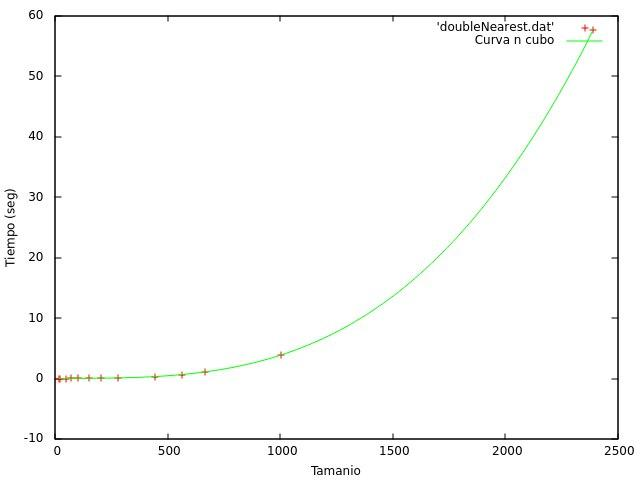
\includegraphics[width=70mm]{graficas/ajustes/doubleNearest}}
\end{figure}
\end{frame}

\section{Resultados}

\begin{frame}\frametitle{ulysses16}
\vspace{-5mm}
\begin{figure}[H]
  \centering
\subfigure[\tiny Ciudades]{\label{graf:ulysses16}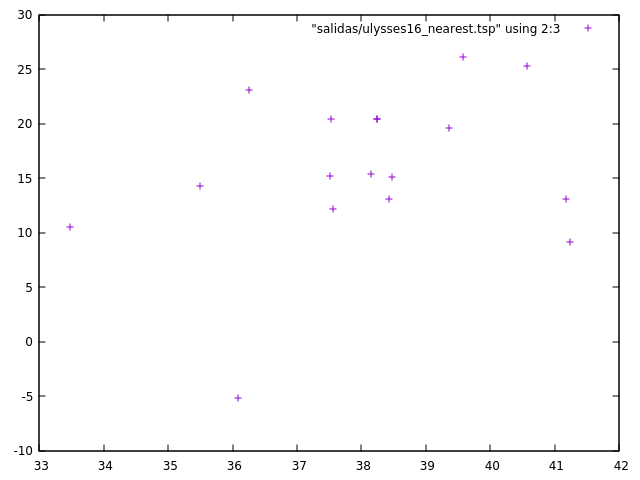
\includegraphics[width=45mm]{graficas/ulysses16}}
\subfigure[\tiny Algoritmo de cercan�a. Peso = 103]{\label{graf:ulysses16_nearest}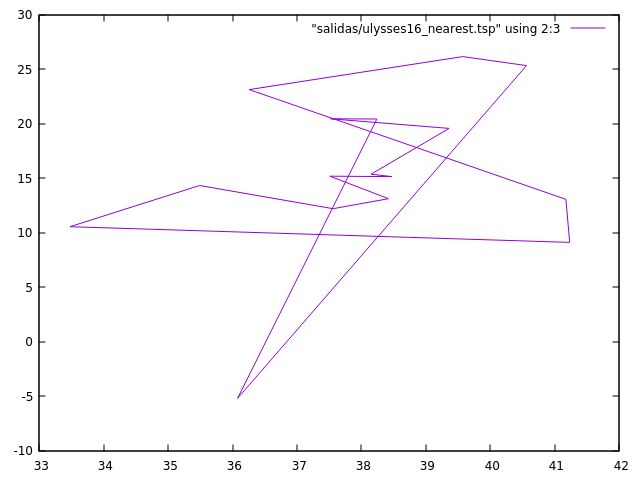
\includegraphics[width=45mm]{graficas/ulysses16_nearest}}
\subfigure[\tiny Algoritmo de inserci�n. Peso = 72]{\label{graf:ulysses16_insertion}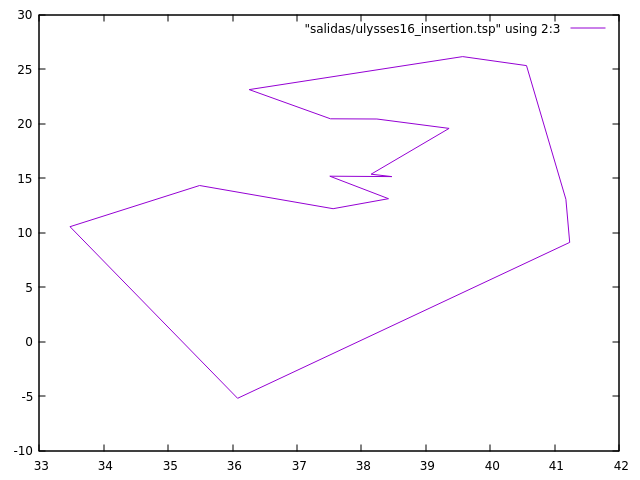
\includegraphics[width=45mm]{graficas/ulysses16_insertion}}
\subfigure[\tiny Algoritmo doubleNearest. Peso = 101]{\label{graf:ulysses16_doubleNearest}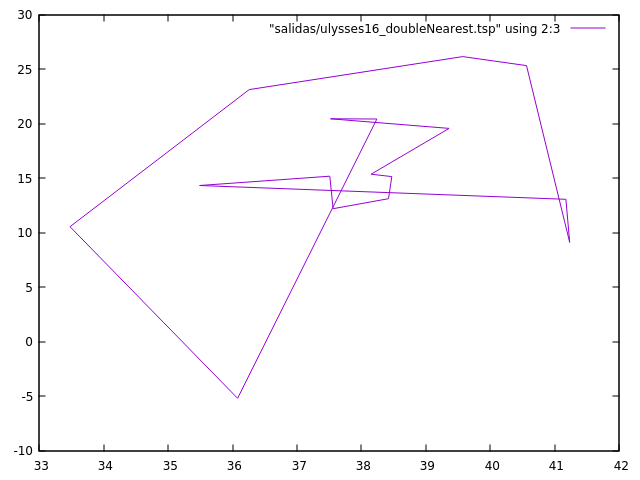
\includegraphics[width=45mm]{graficas/ulysses16_doubleNearest}}
\end{figure}
\end{frame}

\setcounter{subfigure}{0}
\begin{frame}\frametitle{st70}
\vspace{-5mm}
\begin{figure}[H]
  \centering
\subfigure[\tiny Ciudades]{\label{graf:st70}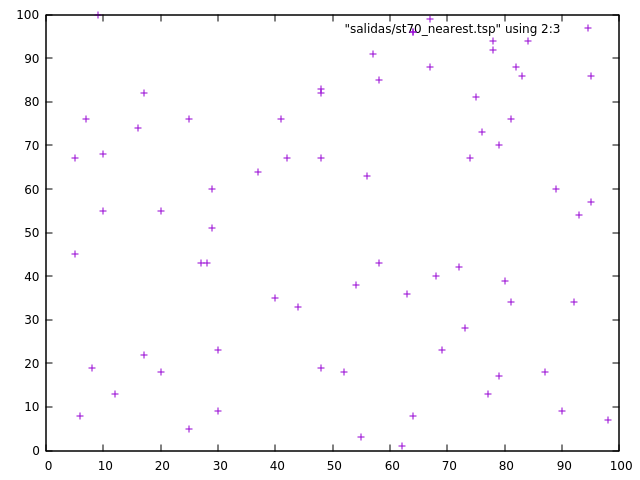
\includegraphics[width=45mm]{graficas/st70}}
\subfigure[\tiny Algoritmo de cercan�a. Peso = 830]{\label{graf:st70_nearest}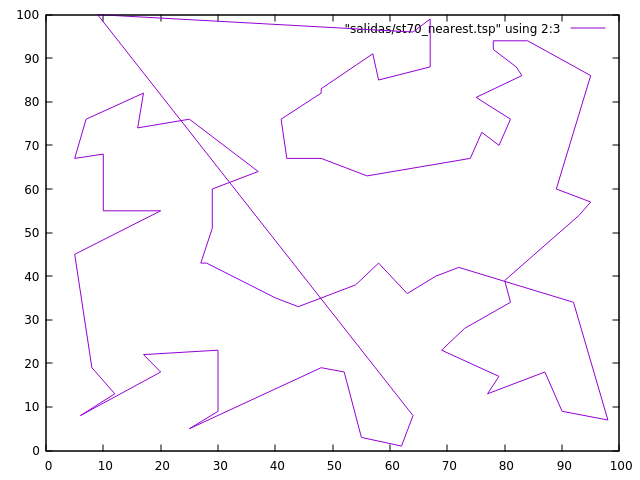
\includegraphics[width=45mm]{graficas/st70_nearest}}
\subfigure[\tiny Algoritmo de inserci�n. Peso = 754]{\label{graf:st70_insertion}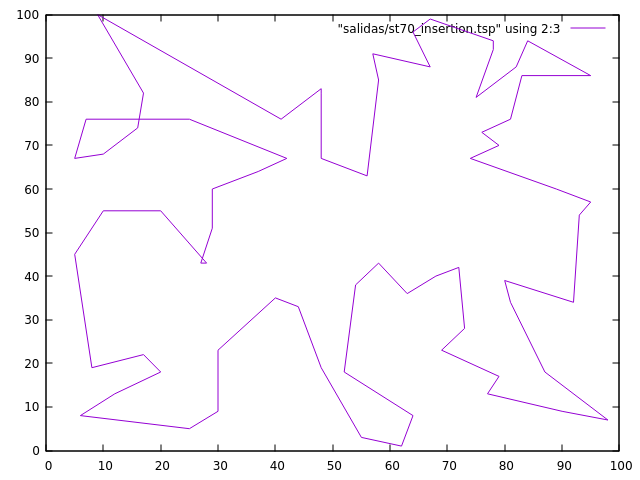
\includegraphics[width=45mm]{graficas/st70_insertion}}
\subfigure[\tiny Algoritmo doubleNearest. Peso = 958]{\label{graf:st70_doubleNearest}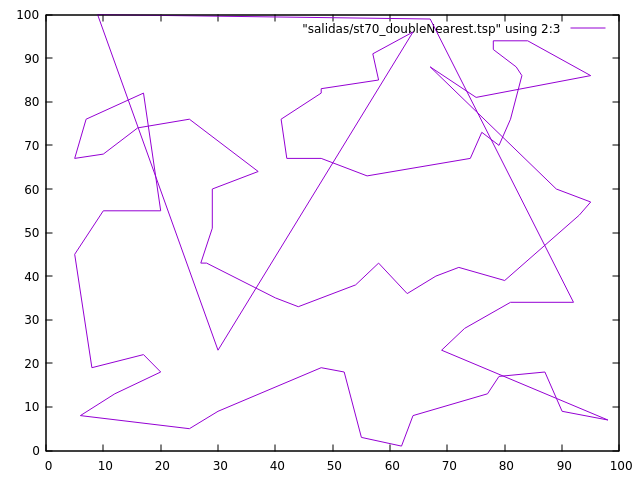
\includegraphics[width=45mm]{graficas/st70_doubleNearest}}
\end{figure}
\end{frame}

\setcounter{subfigure}{0}
\begin{frame}\frametitle{gr202}
\vspace{-5mm}
\begin{figure}[H]
  \centering
\subfigure[\tiny Ciudades]{\label{graf:gr202}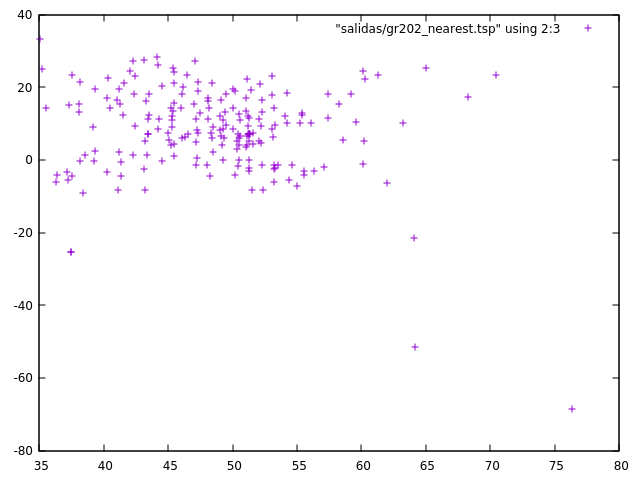
\includegraphics[width=45mm]{graficas/gr202}}
\subfigure[\tiny Algoritmo de cercan�a. Peso = 651]{\label{graf:gr202_nearest}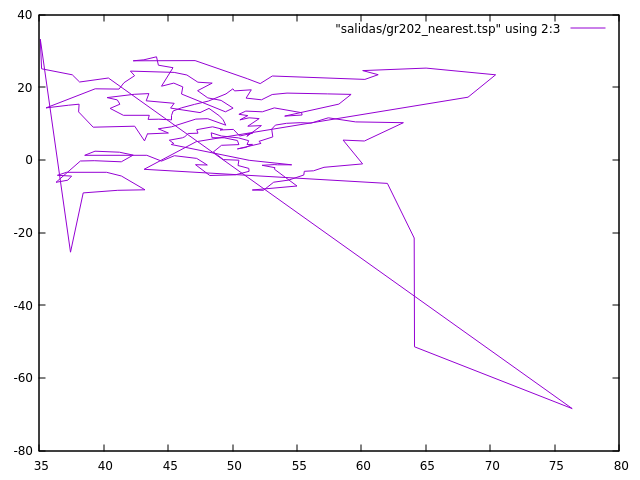
\includegraphics[width=45mm]{graficas/gr202_nearest}}
\subfigure[\tiny Algoritmo de inserci�n. Peso = 554]{\label{graf:gr202_insertion}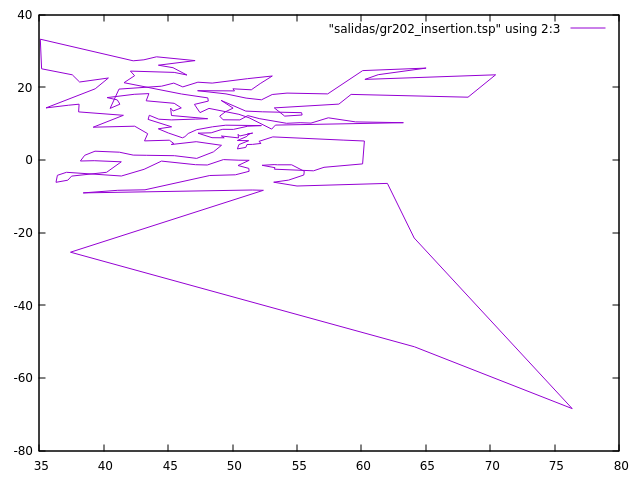
\includegraphics[width=45mm]{graficas/gr202_insertion}}
\subfigure[\tiny Algoritmo doubleNearest. Peso = 688]{\label{graf:gr202_doubleNearest}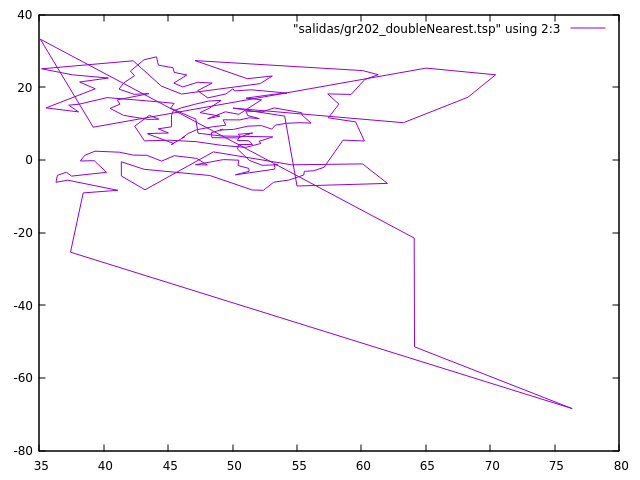
\includegraphics[width=45mm]{graficas/gr202_doubleNearest}}
\end{figure}
\end{frame}

\setcounter{subfigure}{0}
\begin{frame}\frametitle{gr666}
\vspace{-5mm}
\begin{figure}[H]
  \centering
\subfigure[\tiny Ciudades]{\label{graf:gr666}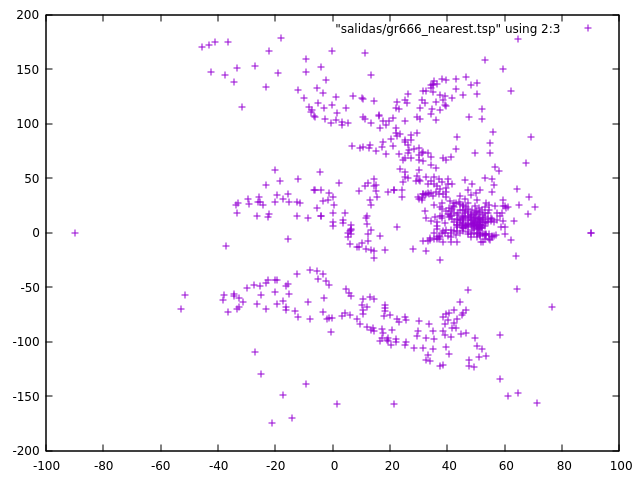
\includegraphics[width=45mm]{graficas/gr666}}
\subfigure[\tiny Algoritmo de cercan�a. Peso = 4046]{\label{graf:gr666_nearest}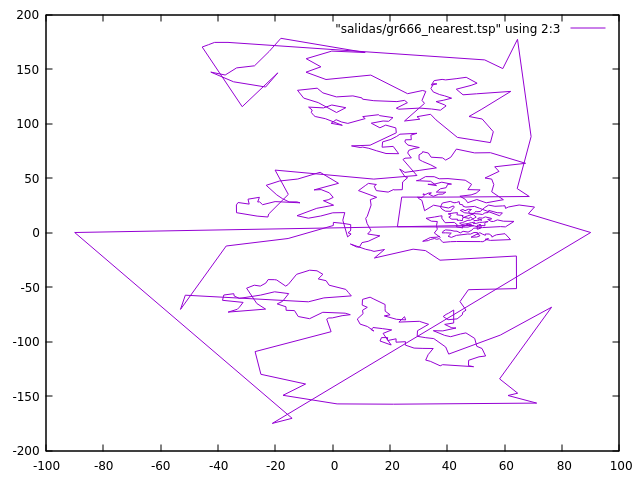
\includegraphics[width=45mm]{graficas/gr666_nearest}}
\subfigure[\tiny Algoritmo de inserci�n. Peso = 3656]{\label{graf:gr666_insertion}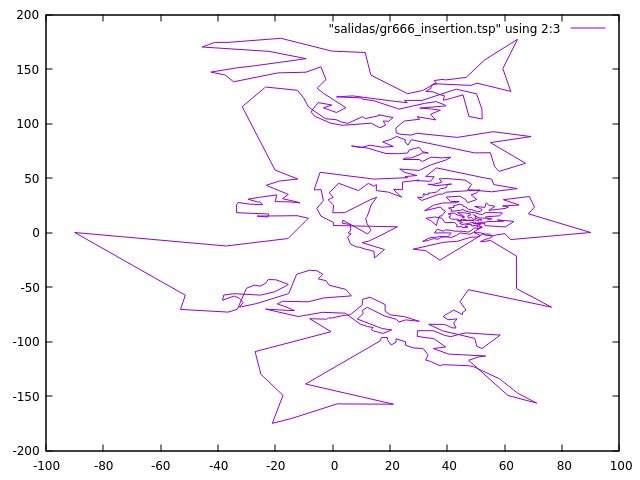
\includegraphics[width=45mm]{graficas/gr666_insertion}}
\subfigure[\tiny Algoritmo doubleNearest. Peso = 4452]{\label{graf:gr666_doubleNearest}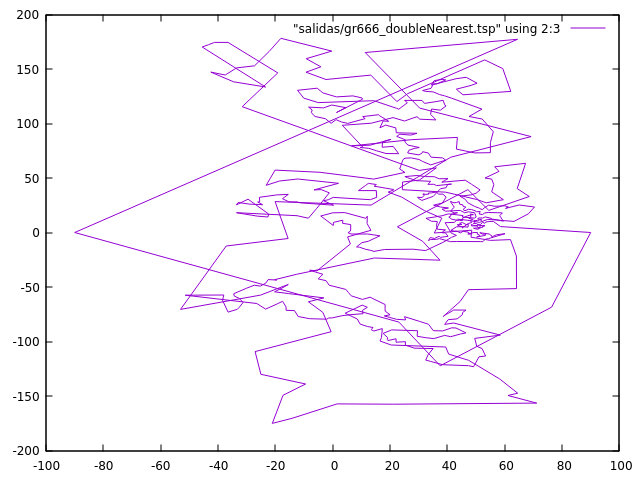
\includegraphics[width=45mm]{graficas/gr666_doubleNearest}}
\end{figure}
\end{frame}

\setcounter{subfigure}{0}
\begin{frame}\frametitle{pr1002}
\vspace{-5mm}
\begin{figure}[H]
  \centering
\subfigure[\tiny Ciudades]{\label{graf:pr1002}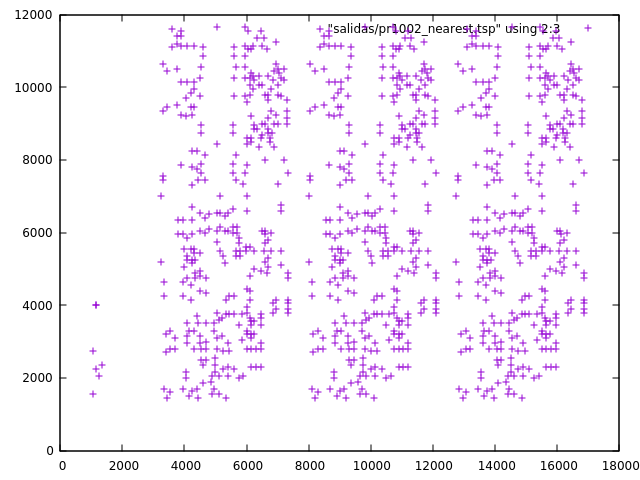
\includegraphics[width=45mm]{graficas/pr1002}}
\subfigure[\tiny Algoritmo de cercan�a. Peso = 331103]{\label{graf:pr1002_nearest}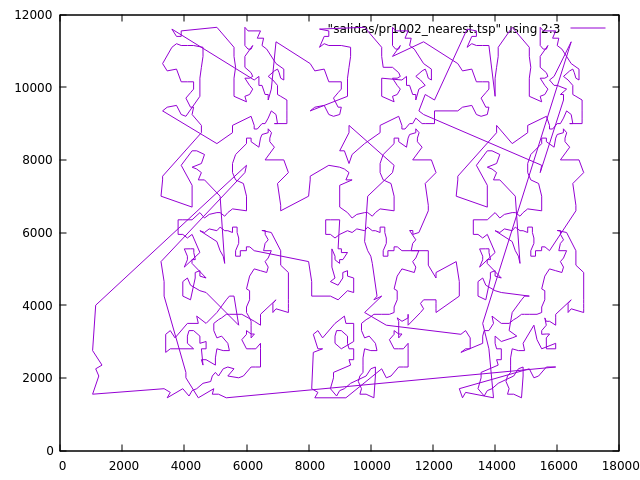
\includegraphics[width=45mm]{graficas/pr1002_nearest}}
\subfigure[\tiny Algoritmo de inserci�n. Peso = 316968]{\label{graf:pr1002_insertion}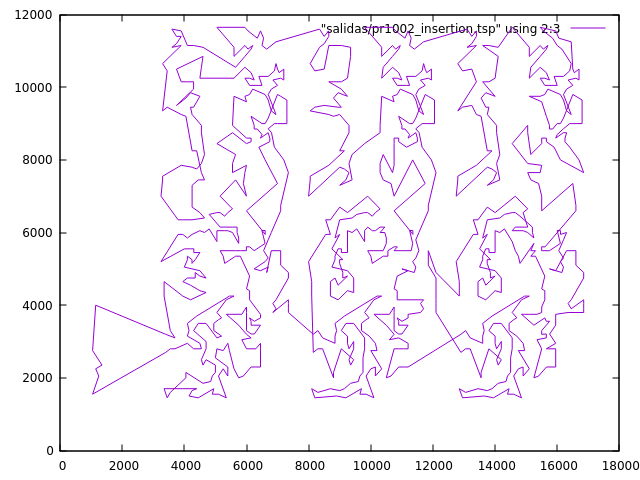
\includegraphics[width=45mm]{graficas/pr1002_insertion}}
\subfigure[\tiny Nuestro algoritmo. Peso = 385020]{\label{graf:pr1002_doubleNearest}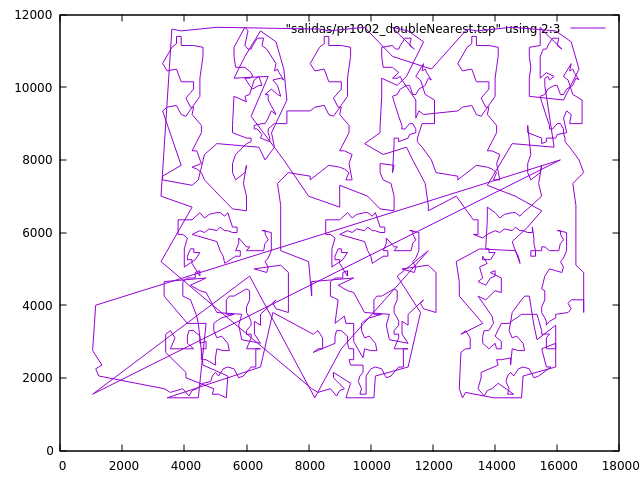
\includegraphics[width=45mm]{graficas/pr1002_doubleNearest}}
\end{figure}
\end{frame}

\begin{frame}\frametitle{Conclusi�n}
   \begin{center}
    \Huge Conclusi�n
  \end{center}
\end{frame}

\end{document}